\subsection{轨道}

定义 5. 设 G 是一个群，E 是一个 G-集，且 \(x \in G\) 。元素 \(y \in E\) 称为在 G 的作用下与 x 共轭，如果存在元素 \(\alpha \in G\) 使得 \(y = \alpha x\) 。x 的共轭元素所成的集合称为 x 在 E 中的轨道。

关系 “y 与 x 共轭” 是一个等价关系。因为 x = ex；若 \(y = \alpha x\) ，则 \(x = \alpha^{-1} y\) ；若 \(y = \alpha x\) 且 \(z = \beta y\) ，则 \(z = \beta \alpha x\) 。轨道是此关系下的等价类。

E 的子集 X 是稳定的，当且仅当它关于共轭关系是饱和的。

G 到 E 的映射 \(\alpha\mapsto\alpha x\) 有时称为由 x 定义的轨道映射。它是 G（其中 G 通过左平移作用于自身）到 E 的一个 G-态射。G 在该映射下的像 G.x 就是 x 的轨道。

称 G 在 E 上自由地作用，如果对所有 \(x \in E\) ，由 x 定义的轨道映射都是单射，或者 G × E 到 E × E 的映射 \((g, x) \mapsto (gx, x)\) 是单射。

例子。(1) 设 G 是一个群，考虑 G 通过内自同构作用于自身。G 的两个元素若在此作用下共轭，则称为在内自同构下共轭，或简称共轭。轨道称为共轭类。类似地，G 的两个子集 H 与 \(H'\) 称为共轭的，如果存在元素 \(\alpha \in G\) 使得 \(H' = \alpha \cdot H \cdot \alpha^{-1}\) ，即它们在 G 通过内自同构作用于自身的这一作用到 \(\mathfrak{P}(G)\) 上的扩张下共轭。

\begin{enumerate}
\def\labelenumi{(\arabic{enumi})}
\setcounter{enumi}{1}
\tightlist
\item
  *在空间 \(\mathbf{R}^n\) 中，点 \(x\) 在正交群 \(\mathbf{O}(n, \mathbf{R})\) 作用下的轨道是半径为 \(\| x \|\) 的欧氏球面。*
\end{enumerate}

E 的两个共轭元素的稳定化子是 G 的共轭子群（第 2 号，命题 2）。

E 在共轭关系下的商集是 E 的轨道集合；有时记为 E/G 或 \(G\backslash E\) 。（有时记号 E/G 保留用于 E 是右 G-集的情形，而记号 \(G\backslash E\) 用于 E 是左 G-集的情形。）

设 G 是一个在集合 E 上右侧作用的群。设 H 是 G 的一个正规子群。群 G 在 E/H 上右侧作用，相应的右作用律为 \((xH, g) \mapsto xHg = xgH\) ；在此作用下，H 平凡地作用，从而得到 G/H 在 E/H 上的一个右作用。设 \(\phi\) 是 E/H 到 E/G 上的典范映射；E/G 的点在 \(\phi\) 下的原像是 G（或 G/H）在 E/H 中的轨道。因此， \(\phi\) 在取商后定义了 \((\mathrm{E}/\mathrm{H})/\mathrm{G} = (\mathrm{E}/\mathrm{H})/(\mathrm{G}/\mathrm{H})\) 到 E/G 上的一个双射，称为典范双射。

设 G（相应地，H）是在集合 E 上左作用（相应地，右作用）的群。假设 G 与 H 在 E 上的作用可交换，即

\[
(g. x). h = g. (x. h) \quad \text { for } g \in \mathrm{G}, x \in \mathrm{E} \text { and } h \in \mathrm{H}.
\]

H 在 E 上的作用也可视为 H 的反群 \(H^{0}\) 在 E 上的左作用。于是由 §4，第 9 号，命题 12 可知，把元素 \((g, h) \in G \times H^{0}\) 对应到 E 到自身的映射 \(x \mapsto g \cdot x \cdot h\) 的映射，是 \(G \times H^{0}\) 在 E 上的一个左作用。元素 \(x \in E\) 在此作用下的轨道是集合 GxH。这些轨道的集合记为 \(G\backslash E/H\) 。另一方面，G（相应地，H）的作用与关于 H（相应地，G）的作用的共轭关系相容，且轨道集合 \(G\backslash(E/H)\) （相应地，\((G\backslash E)/H\) ）等同于 \(G\backslash E/H\) ：在图中

\pandocbounded{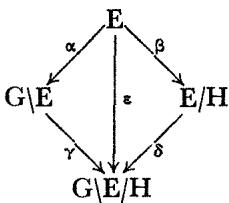
\includegraphics[keepaspectratio]{images/part001_b92675b5.jpg}}

（其中 \(\alpha, \beta, \gamma, \delta, \varepsilon\) 表示取商的典范映射）， \(\gamma \circ \alpha = \delta \circ \beta = \varepsilon\) 。

设 G 为一个群，H 为 G 的子群。考虑 H 通过右平移在 G 上的右作用（第 1 号，例 2）。轨道集合 G/H 是模 H 的左陪集集合；注意 G 依法则 \((g, xH) \mapsto gxH\) 在 G/H 上左作用（参见第 5 号）。类似地，模 H 的右陪集集合是 H 通过左平移在 G 上左作用的轨道集合 \(H\backslash G\) 。若 K 是 G 的包含 H 的子群，且 \(\Gamma\) 是模 H 的左（相应地，右）陪集，则 \(\Gamma K\) （相应地，\(K\Gamma\) ）是模 K 的左（相应地，右）陪集。映射 \(\Gamma \mapsto \Gamma K\) （相应地，\(\Gamma \mapsto K\Gamma\) ）称为 G/H 到 G/K（相应地，\(H\backslash G\) 到 \(K\backslash G\) ）的典范映射。它是满射。

设 G 为一个群，H 和 K 为 G 的两个子群。令 H 通过左平移在 G 上左作用，K 通过右平移在 G 上右作用；这两个作用可交换，故可考虑集合 \(H\backslash G/K\) 。\(H\backslash G/K\) 的元素称为 G 模 H 与 K 的双陪集。当 K = H 时，简称模 H 的双陪集。G/H 到 \(H\backslash G/H\) 上的典范映射是双射，当且仅当 H 是 G 的正规子群。

